\subsection{Verfahren im Überblick}
\begin{frame}
Aufbereitung des Bildausschnittes für die Gesichtsanalyse.
\begin{itemize}
	\item<1-> Bicubic-Skalierung:\\
	Funktion 3. Grades über $4\times 4$ Pixel
	\item<1-> Lanczos-Skalierung:\\
	Sinc-Funktion über $8\times 8$ Pixel
	\item<1-> Linear-Skalierung:\\
	Funktion 1. Grades über umliegende Pixel
	\item<1-> Nearest-Neighbor-Skalierung:\\
	Nächstgelegener Farbwert
\end{itemize}
		\begin{center}
			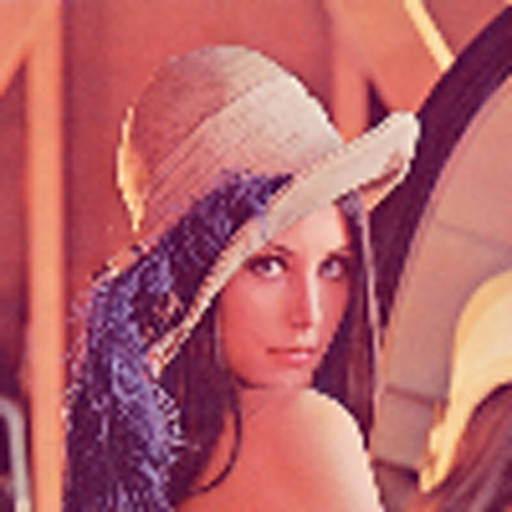
\includegraphics[width=0.24\linewidth]{img_Skal/lena100_CUBIC}
			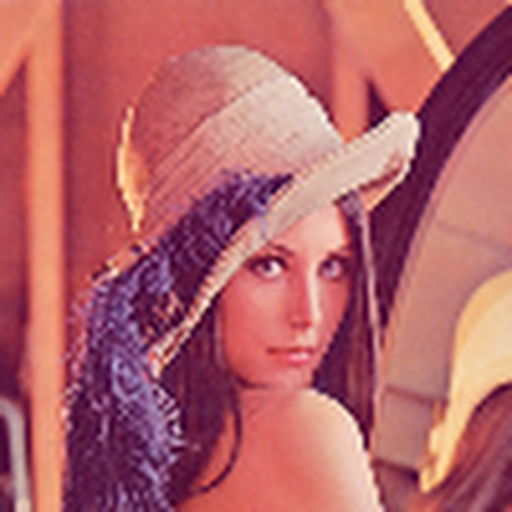
\includegraphics[width=0.24\linewidth]{img_Skal/lena100_LANCZOS4}
			
\includegraphics[width=0.24\linewidth]{img_Skal/lena100_LINEAR}
			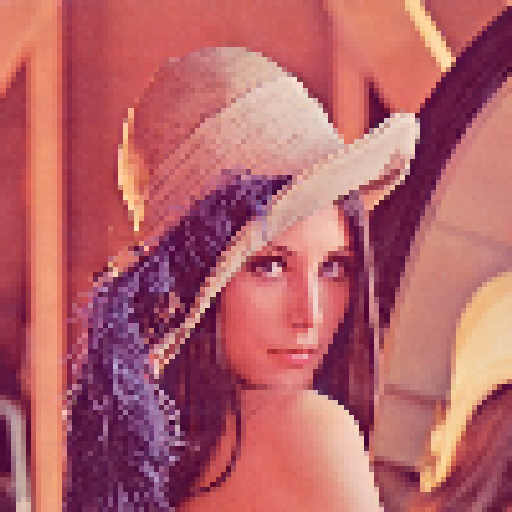
\includegraphics[width=0.24\linewidth]{img_Skal/lena100_NN}
		\end{center}
\end{frame}
\subsection{Auswirkung auf die Detektionsrate}
\begin{frame}
\begin{center}
	\footnotesize{LFW (schwarz, Gesichter 95 Pixel) und BIWI (rot,  Gesichter 78 Pixel)}\\
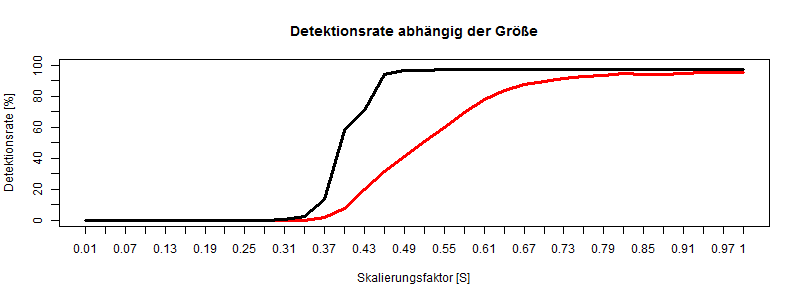
\includegraphics[width=0.8\linewidth]{img_Skal/Gesicht_Rate}\\
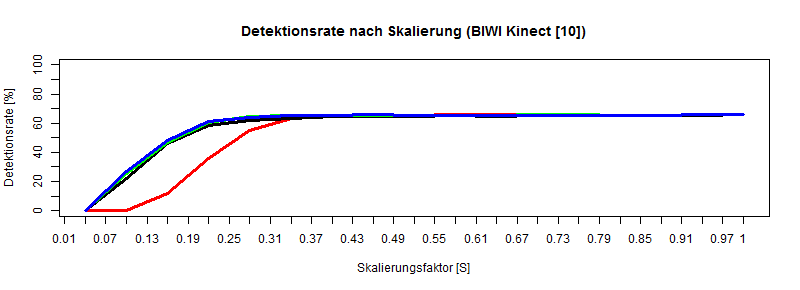
\includegraphics[width=0.8\linewidth]{img_Skal/Resize_Rate_Ges}\\
\footnotesize{Bicubic (blau), Lanczos (grün), Linear (schwarz), N.-Neighbor (rot)}
\end{center}
\end{frame}